\documentclass[a4paper,12pt]{article}

\usepackage[
    left=2cm,
    right=2cm,
    top=3cm,
    bottom=3cm
]{geometry}

\usepackage[utf8]{inputenc}
\usepackage[czech]{babel}
\usepackage[T1]{fontenc}
\usepackage{graphicx}
\usepackage{array}
\usepackage{booktabs}
\usepackage{tabularx}
\usepackage{makecell}
\usepackage{float}
\usepackage{newunicodechar}
\usepackage{url}
\usepackage{siunitx}
\usepackage{listings}
\usepackage{xcolor}
\usepackage{diagbox}
\usepackage{hyperref}

\usepackage{fancyhdr}
\pagestyle{fancy}

\fancyhf{}
\fancyhead[L]{Měření na Peltierově článku – laboratorní cvičení}
\fancyhead[R]{Pavel Pernička}
\fancyfoot[C]{\thepage}

\fancypagestyle{firstpage}{
    \fancyhf{}
    \renewcommand{\headrulewidth}{0pt}
    \renewcommand{\footrulewidth}{0pt}
    \fancyfoot[C]{\thepage}
}

\newcommand{\unitC}{\,^\circ\mathrm{C}}
\newcommand{\unitV}{\,\mathrm{V}}
\newcommand{\unitA}{\,\mathrm{A}}
\newcommand{\units}{\,\mathrm{s}}
\newcommand{\unitmin}{\,\mathrm{min}}

\newcommand{\centered}[1]{\begin{tabular}{l} #1 \end{tabular}}

\addto\captionsczech{\renewcommand{\refname}{Seznam použité literatury}}
\addto\captionsczech{\renewcommand{\figurename}{\textbf{Obrázek}}}
\addto\captionsczech{\renewcommand{\tablename}{\textbf{Tabulka}}}
\renewcommand{\lstlistingname}{\textbf{Kód}}

\lstset{
    language=Python,
    basicstyle=\ttfamily\footnotesize,
    keywordstyle=\color{blue},
    commentstyle=\color{gray},
    stringstyle=\color{red},
    numbers=left,
    numberstyle=\tiny\color{gray},
    stepnumber=1,
    breaklines=true,
    frame=single
}

\begin{document}
\thispagestyle{firstpage}

\vspace*{\fill}
\begin{center}
\renewcommand{\arraystretch}{1.75}

\begin{tabularx}{\textwidth}{|X|X|X|}
    \hline
    \multicolumn{1}{|c|}{\rule{0pt}{2.25cm} 
\includegraphics[height=2cm]{img/ctu_logo.png}}
    & \multicolumn{2}{c|}{\makecell{\textbf{KATEDRA FYZIKY}}} \\
    \hline
    \multicolumn{3}{|c|}{\Large \textbf{\centered{LABORATORNÍ CVIČENÍ Z FYZIKY}}} \\
    \hline
    \multicolumn{2}{|X}{\small{Jméno} \newline \textbf{Pavel Pernička}}
    & \multicolumn{1}{|X|}{\small{Datum měření} \newline \textbf{14.10.2025}} \\
    \hline
    {\small{Semestr} \newline \textbf{Zimní 2025}}
    & {\small{Ročník} \newline \textbf{2.}}
    & {\small{Datum odevzdání} \newline \textbf{21.11.2025}} \\
    \hline
    {\small{Stud. skupina} \newline \textbf{6}}
    & {\small{Lab. skupina} \newline \textbf{1061}}
    & {\small{Klasifikace} \newline} \\
    \hline
    \multicolumn{3}{|c|}{\rule{0pt}{1cm}} \\
    \hline
    \multicolumn{1}{|X|}{\small{Číslo úlohy \newline \textbf{6}}}
    & \multicolumn{2}{|p{8cm}|}{\small{Název úlohy \newline \textbf{Měření na Peltierově článku}}} \\
    \hline
\end{tabularx}

\end{center}
\vspace*{\fill}

\newpage
\section{Úkol měření}
V této práci měříme vlastnosti Peltierova článku v různých režimech s následujícím zadáním:
\begin{itemize}
\item V režimu termoelektrického generátoru (TEG):
\begin{enumerate}
    \item změřte závislost termoelektrického napětí na teplotě a vyneste ji do grafu,
    \item z naměřené závislosti vypočtěte Seebeckův koeficient,
    \item vypočítejte účinnost Peltierova článku v režimu TEG a vypočtenou hodnotu porovnejte s účinností vratně pracujícího tepelného stroje.
\end{enumerate}

\item V režimu termoelektrického chladiče (TEC) a termoelektrického ohřívače (TEH):
\begin{enumerate}
    \item změřte časovou závislost teploty na obou stranách Peltierova článku a vyneste ji do grafu.
\end{enumerate}
\end{itemize}

\section{Seznam použitých měřicích přístrojů}
\begin{itemize}
    \item 2x digitální teploměry
        \begin{itemize}
            \item Označení: GMH 1170
            \item Rozsah: $-65\unitC$ -- $199\unitC$
            \item Přesnost: $\pm 0,05\ \%$
            \item Rozlišení: $0,1\unitC$
        \end{itemize}
    \item Multimetr MY-65 v režimu voltmetru
        \begin{itemize}
            \item Rozsah: $20\unitV$
            \item Přesnost: $\pm 0,1\ \%$
            \item Rozlišení: $1\ \unit{mV}$
        \end{itemize}
    \item Multimetr MY-65 v režimu ampérmetru
        \begin{itemize}
            \item Rozsah: $10\ \unitA$
            \item Přesnost: $\pm 0,8\ \%$
            \item Rozlišení: $1\ \unit{mA}$
        \end{itemize}
\end{itemize}

\newpage
\section{Peltierův článek jako zdroj elektrické energie}

\subsection{Postup}
\begin{enumerate}
    \item Zapojíme do napájení čerpadlo v chladicím okruhu, aby v něm cirkulovala studená voda z rezerovoáru (Obrázek \ref{fig:aparatura}).
    \item K terminálům Peltierova článku paralelně zapojíme voltmetr a přichystáme si jeden kontakt pro budoucí dočasné paralelní zapojení ampérmetru.
    \item Do teploměrů zapojíme termistory.
    \item Ohřejeme vodu a nalijeme ji do nádoby připojené k termočlánku.
    \item Až přestane teplota na teplé straně článku růst, odečítáme po 30 vteřinách napětí na článku, teploty z obou termistorů a zkratový proud.
\end{enumerate}

\begin{figure}[H]
    \centering
    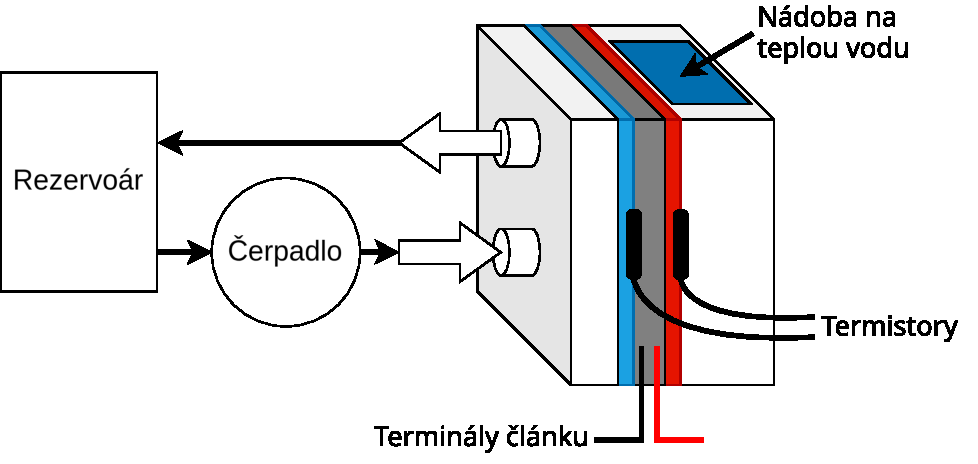
\includegraphics[width=0.95\textwidth]{img/aparatura.pdf}
    \caption{Schematický nákres použité aparatury}
    \label{fig:aparatura}
\end{figure}

\subsection{Naměřené hodnoty}

\begin{table}[H]
\centering
\renewcommand{\arraystretch}{1.5}
\begin{tabular}{|c|c|c|c|c|c|}
\hline
Čas \textbf{[s]} & \textbf{$U_n$ [V]} & \textbf{$I_n$ [A]} & \textbf{$T_S$ [°C]} & \textbf{$T_H$ [°C]} & \textbf{$\Delta T$ [°C]} \\
\hline
0   & 1,21 & 0,131 & 24,8 & 58,3 & 33,5 \\
30  & 1,16 & 0,127 & 24,9 & 57,4 & 32,5 \\
60  & 1,13 & 0,122 & 25,0 & 56,3 & 31,3 \\
90  & 1,07 & 0,117 & 25,0 & 55,1 & 30,1 \\
120 & 1,03 & 0,112 & 25,0 & 53,6 & 28,6 \\
150 & 0,98 & 0,107 & 24,9 & 52,3 & 27,4 \\
180 & 0,94 & 0,102 & 24,9 & 51,2 & 26,3 \\
210 & 0,90 & 0,098 & 24,8 & 50,0 & 25,2 \\
240 & 0,85 & 0,093 & 24,7 & 48,9 & 24,2 \\
270 & 0,82 & 0,090 & 24,6 & 48,0 & 23,4 \\
300 & 0,79 & 0,086 & 24,6 & 47,1 & 22,5 \\
330 & 0,76 & 0,083 & 24,5 & 46,2 & 21,7 \\
360 & 0,73 & 0,080 & 24,4 & 45,3 & 20,9 \\
390 & 0,70 & 0,077 & 24,3 & 44,3 & 20,0 \\
420 & 0,68 & 0,074 & 24,2 & 43,7 & 19,5 \\
\hline
\end{tabular}
\caption{Naměřené hodnoty, $U_n$ = napětí na prázdno, $I_n$ = proud nakrátko, $T_S, T_H$ = teploty na studené a horké straně článku}
\label{tab:teg_values_teg}
\end{table}

\subsection{Graf a Seebeckův koeficient}
Z naměřených hodnot a spočítaného teplotního rozdílu $\Delta T$ jsme vytvořili graf \ref{fig:graf_seebeck} ukazující závislost $U_n$ na $\Delta T$. Pomocí metody nejmenších čtverců jsme proložili datové body polynomem prvního řádu $0,03775 x - 0,05759$. Zanedbáme-li skutečnost, že závislost není ve větším měřítku čistě lineární, můžeme přímo ze směrnicového členu zjistit Seebeckův koeficient $\alpha=37,75\ \unit{mV}\cdot~\unitC^{-1}.$

\begin{figure}[H]
    \centering
    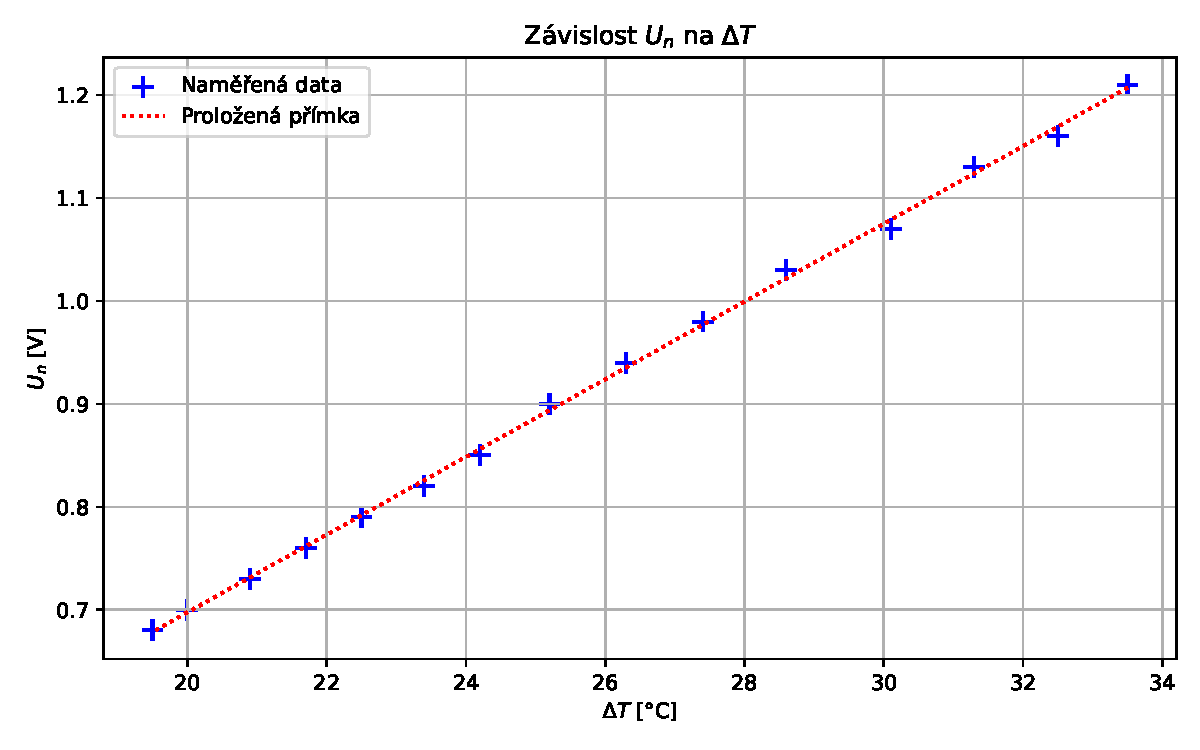
\includegraphics[width=1\textwidth]{img/graf_peltier_zdroj.pdf}
    \caption{Graf závislosti napětí na termočlánku na rozdílu teplot jeho stran, body proloženy polynomem prvního řádu}
    \label{fig:graf_seebeck}
\end{figure}

\subsection{Výpočet účinnosti}
Ze zadání známe vzorec pro výpočet účinnosti termoelektrického generátoru:
$$\eta_{TEG} = \frac{P_E}{P_H}$$
Pro její složky platí navíc tyto vztahy:
$$P_E = \frac{1}{4} U_0 I_K \quad \quad P_H \approx \frac{\Delta Q_H}{\Delta T} = \frac{C_{celk} (T_{H1} - T_{H_2})}{t_1 - t_2}$$
Kde:
\begin{itemize}
    \item $\eta_{TEG}$ je účinnost Peltierova článku v režimu TEG
    \item $P_E$ je odhad teoretického maximálního výkonu dodávaného článkem do zátěže
    \item $P_H$ je tepelný výkon procházející teplou stranou do článku (počítáme s tím, že veškeré teplo z nádobky s horkou vodou prochází článkem)
    \item $C_{celk} = 1121 J K^{-1}$ je celková tepelná kapacita nádobky s vodou
    \item $T_{H1}, T_{H2}$ jsou teploty na horké straně v časech $t_1, t_2$
\end{itemize}
Pokud do vztahů výše dosadíme hodnoty z prvního časového bodu měření, vypočítáme:
$$P_E = \frac{1,21 \cdot 0,131}{4} = 0,0396\ \unit{W} \quad \quad P_H \approx \frac{1121 (58,3 - 57,4)}{30} = 33,6299\ \unit{W}$$
Tedy:
$$\eta_{TEG} = 0,1178\ \%$$
Dále spočítáme teoretickou účinnost pro ideální situaci vratně pracujícího tepelného stroje pomocí vztahu:
$$\eta'_{TEG} = \frac{T_H - T_S}{T_H} = 10,1071\ \%$$
Když obě účinnosti srovnáme, zjistíme, že reálná účinnost tvoří jen zhruba $1,16\ \%$ maximální účinnosti vratně pracujícího tepelného stroje. 

\subsection{Nejistoty}
Pro Seebeckův koeficient musíme zahrnout přístrojovou nejistotu typu B pro použitý voltmetr, kterým jsme měřili $U_n$. Tu stanovíme z parametrů přístroje následovně:
$$u_b(U_n) = \frac{U_n \cdot \frac{0.1}{100} + 0,003}{\sqrt{3}}$$
Spočtením pro naměřené hodnoty získáváme finální výsledek:
$$\alpha = (37,8 \pm 2)\ \unit{mV}\cdot \unitC^{-1}$$

Pro účinnost, který závisí na více veličinách, použijeme nejistotu typu C danou následujícím vztahem:
$$u_c = \sqrt{\sum_{i=1}^{N}{a_i}} = \sqrt{\sum_{i=1}^{N}{\left(\frac{\partial \eta}{\partial x_i}\right)\cdot u_b^2(x_i)}}$$

kde:
\begin{itemize}
    \item $x_i$ je veličina na které závisí účinnost,
    \item $u_b(x_i)$ jsou přístrojové nejistoty měření dané veličiny. Ty máme vypočítané v předchozích krocích. Jako nejistotu pro časové údaje zvolíme cca 2 sekundy, jakožto reakční čas pozorovatele.
\end{itemize}

Vypočítáme parciální derivace a dosadíme nejistoty:

$$a_1 = \left( \frac{\partial \eta}{\partial U_n} \right) \cdot u_b^2(U_n) = \frac{1}{4} \frac{I_n(t_2-t_1)}{C_{celk} (T_{H1} - T_{H_2})} \cdot u_b^2(U_n)$$

$$a_2 = \left( \frac{\partial \eta}{\partial I_n} \right) \cdot u_b^2(U_n) = \frac{1}{4} \frac{U_n(t_2-t_1)}{C_{celk} (T_{H1} - T_{H_2})} \cdot u_b^2(I_n)$$

$$a_3 = \left( \frac{\partial \eta}{\partial T_{H1}} \right) \cdot u_b^2(U_n) = -\frac{1}{4} \frac{U_n I_n(t_2-t_1)}{C_{celk} (T_{H1} - T_{H_2})^2} \cdot u_b^2(T_{H1})$$

$$a_4 = \left( \frac{\partial \eta}{\partial T_{H2}} \right) \cdot u_b^2(U_n) = \frac{1}{4} \frac{U_n I_n(t_2-t_1)}{C_{celk} (T_{H1} - T_{H_2})^2} \cdot u_b^2(T_{H2})$$

$$a_5 = \left( \frac{\partial \eta}{\partial t_1} \right) \cdot u_b^2(U_n) = \frac{1}{4} \frac{U_n I_n}{C_{celk} (T_{H1} - T_{H_2})} \cdot u_b^2(t_1) $$

$$a_6 = \left( \frac{\partial \eta}{\partial t_2} \right) \cdot u_b^2(U_n) = \frac{1}{4} \frac{U_n I_n}{C_{celk} (T_{H1} - T_{H_2})} \cdot u_b^2(t_2)$$

Pomocí skriptu spočítáme, že účinnost má následující nejistotu:

$$\eta_{TEG} = (0,12 \pm 0,02)\ \unit{\%}$$

Nejistotu pro maximální účinnost vratně pracujícího tepelného stroje vypočítáme obdobným způsobem pomocí těchto parciálních derivací:
$$\frac{\partial \eta'}{T_H} = \frac{T_S}{T_H^2}
\quad \quad
\frac{\partial \eta'}{T_S} = -\frac{1}{T_H}$$

Dosazením získáváme:

$$\eta'_{TEG} = (10,11 \pm 0,12)\ \unit{\%}$$

\section{Peltierův článek jako chladicí stroj a ohřívač}
\subsection{Postup}
\begin{itemize}
    \item Pro chladicí stroj:
        \begin{enumerate}
        \item Nádobu na straně článku naplníme vodou o pokojové teplotě
        \item Zapojíme Peltierův článek do napájení, zdroj nastavíme tak, aby byl proud omezen na $I_{max} = 4\ \unit{A}$
        \item V minutových intervalech měříme teploty na obou stranách článku
    \end{enumerate}
    \item Pro ohřívač opakujeme stejný postup při opačné polaritě s tím, že navíc hlídáme, aby teplota na horké straně článku nepřekročila $T_{max} = 70\ \unitC$.
    
\end{itemize}

\subsection{Naměřené hodnoty}

\begin{table}[H]
\centering
\renewcommand{\arraystretch}{1.5}

\begin{minipage}{0.47\textwidth}
\centering
\renewcommand{\arraystretch}{1.5}
\begin{tabular}{|c|c|c|}
\hline
Čas \textbf{[min]} & \textbf{$T_S$ [$\unitC$]} & \textbf{$T_H$ [$\unitC$]} \\
\hline
$0$ & $26,1$ & $23,2$  \\
$1$ & $23,2$ & $24,5$  \\
$2$ & $22,2$ & $26,6$  \\
$3$ & $21,1$ & $26,8$  \\
$4$ & $20,3$ & $26,7$  \\
$5$ & $19,4$ & $26,8$  \\
$6$ & $18,7$ & $26,6$  \\
$7$ & $18,1$ & $26,6$  \\
$8$ & $17,4$ & $26,6$  \\
$9$ & $16,9$ & $26,5$  \\
$10$ & $16,3$ & $26,5$  \\
$11$ & $15,7$ & $26,5$  \\
$12$ & $15,3$ & $26,4$  \\
$13$ & $14,8$ & $26,3$  \\
$14$ & $14,4$ & $26,3$  \\
$15$ & $13,8$ & $26,2$  \\
\hline
\end{tabular}
\caption{Naměřené teploty na stranách článku v režimu TEC při $I = 2,18\unitA$, $U~=~6,3\unitV$}
\label{tab:cooling_values}
\end{minipage}
\hfill
\begin{minipage}{0.47\textwidth}
\centering
\renewcommand{\arraystretch}{1.5}
\begin{tabular}{|c|c|c|}
\hline
\textbf{Čas [$\unitmin$]} & \textbf{$T_S$ [$\unitC$]} & \textbf{$T_H$ [$\unitC$]} \\
\hline
0  & 22,3 & 22,4 \\
1  & 19,8 & 28,7 \\
2  & 19,8 & 30,8 \\
3  & 19,8 & 31,8 \\
4  & 20,0 & 33,0 \\
5  & 20,1 & 33,9 \\
6  & 20,1 & 35,0 \\
7  & 20,3 & 35,7 \\
8  & 20,3 & 36,4 \\
9  & 20,4 & 37,2 \\
10 & 20,5 & 37,8 \\
11 & 20,6 & 38,6 \\
12 & 20,7 & 39,3 \\
13 & 20,7 & 39,9 \\
14 & 20,8 & 40,6 \\
\hline
\end{tabular}
\caption{Naměřené teploty na stranách článku v režimu TEH při $I = 2{,}17\unitA$, $U~=~7{,}11\unitV$.}
\label{tab:heating_values}
\end{minipage}
\end{table}

\subsection{Grafy}

\begin{figure}[H]
    \centering

    % První graf (chlazení)
    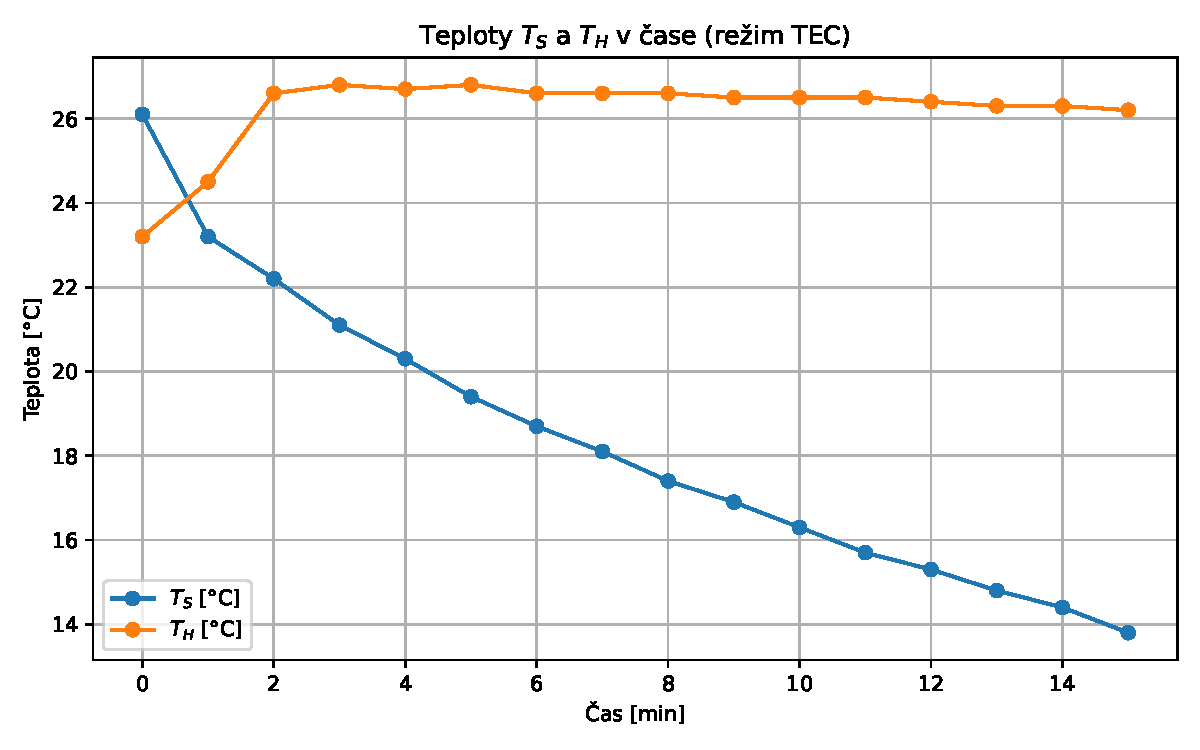
\includegraphics[width=\textwidth, height=0.44\textheight, keepaspectratio]{img/graf_peltier_chlazeni.pdf}

    \vspace{0.5cm}

    % Druhý graf (ohřev)
    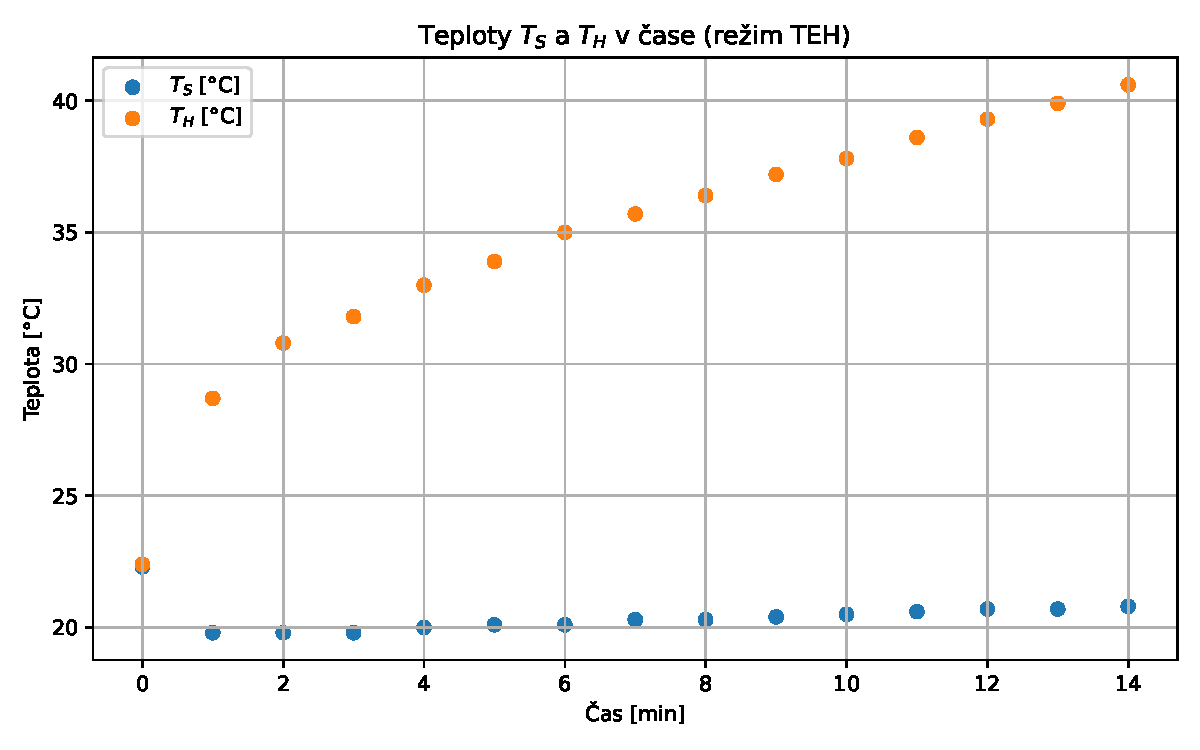
\includegraphics[width=\textwidth, height=0.44\textheight, keepaspectratio]{img/graf_peltier_ohrev.pdf}

    \caption{Grafy vývoje teplot na stranách termočlánku v čase}
    \label{fig:graf_spolecny}
\end{figure}

\section{Závěr}
V laboratorní úloze jsme pomocí měření teplot, napětí a zkratového proudu zjistili Seebeckův koeficient, který nám v režimu termoelektrického generátoru udává závislost napětí naprázdno na rozdílu teplot studené a teplé strany. Jeho hodnota je:

$$\alpha = (37,8 \pm 2)\ \unit{mV}\cdot \unitC^{-1}$$
Dále jsme se přesvědčili o poměrně nízké efektivitě Peltierova článku, jakožto generátoru elektrické energie. Ta činí jen:

$$\eta_{TEG} = (0,12 \pm 0,02)\ \unit{\%}, $$
což je jen necelých $1,16\ \%$ účinnosti, které dosáhne optimální vratně pracující tepelný stroj ve stejných podmínkách (ten by měl mít $\eta'_{TEG} = (10,11 \pm 0,12)\ \unit{\%}$). 

V režimu termoelektrického chladiče se nám podařilo dosáhnout nejnižší teploty $T_s~=~13,8 \unitC$ (tedy $T_{start}-T_{end} = 12,3 \unitC$), ale jak lze vidět z tendence grafu, pokud bychom článek nechali běžet déle, nebo měli nastavený zdroj blíže k maximálním hodnotám pro článek, dosáhli bychom ještě nižší teploty.

V režimu ohřívače byla změna teploty v čase při podobných parametrech vyšší, než u chladiče. Zde se nám podařilo dosáhnout nejvyšší teploty $T_h = 40,6 \unitC$, tedy $T_{start}-T_{end} = 18,2 \unitC$). Tento děj je rychlejší, jelikož kromě samotného čerpání tepla dochází také ke vzniku Jouleova tepla uvnitř samotných polovodičových prvků, které ohřev urychluje.

\section{Přílohy}
Jupyter notebook pro výpočty a kreslení grafu: jako příloha nebo dostupné online:  \url{https://colab.research.google.com/drive/1mV62pdKovMqddPFaJD4j_541HQQD1n1g?usp=sharing}

\begin{thebibliography}{}

    \bibitem{zadani}
    Milan Červenka. \textit{Měření na Peltierově článku}. Laboratorní úloha, 2015. Dostupné online: \url{https://planck.fel.cvut.cz/praktikum/downloads/navody/peltier.pdf}.

    \bibitem{skripta}
    Michal Bednařík. \textit{Studijní texty k předmětu Fyzika 2}.
    
    \bibitem{zpracdat}
    Milan Červenka. \textit{Zpracování fyzikálních měření}. Studijní text pro fyzikální praktikum, 2020. Dostupné online: \url{https://planck.fel.cvut.cz/praktikum/downloads/navody/zpracdat.pdf}.

\end{thebibliography}

\end{document}
